% fig10_meta_lattice — n=6 divisor lattice + alien_index chain.
% Standalone TikZ; compiled to figures/fig10_meta_lattice.pdf.
% Comparison (verifiable arithmetic vs UNPROVEN physics across the chain)
% => chart (user hard rule). Data: Appendix H, UFO/meta/{lattice-policy,
% limit-breakthrough}.md.
\documentclass[tikz,border=6pt]{standalone}
\usepackage{tikz}
\usetikzlibrary{positioning,arrows.meta}
\usepackage{amssymb}
\usepackage{xcolor}
\begin{document}
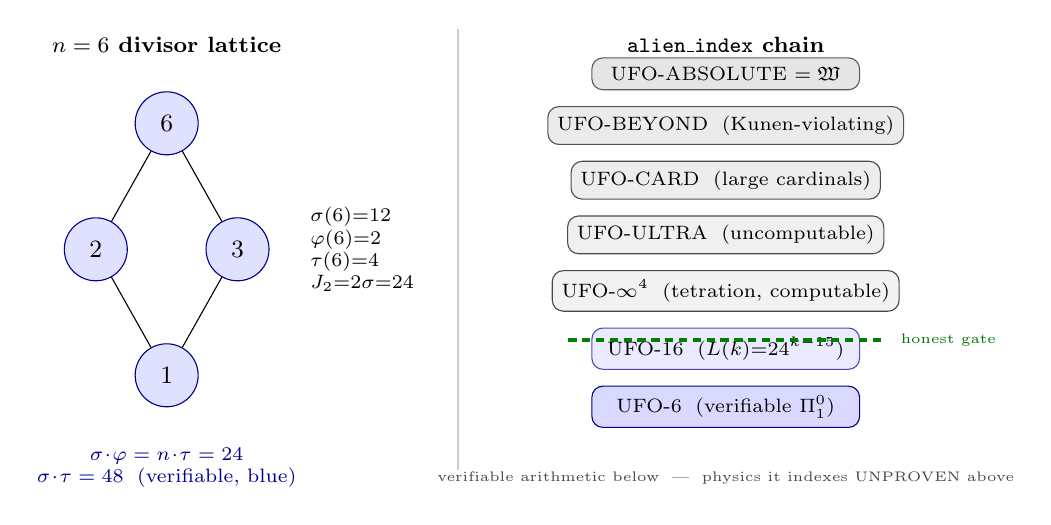
\begin{tikzpicture}[
  dn/.style={draw=blue!55!black, fill=blue!12, circle, minimum size=8mm, font=\small},
  >=Stealth,
]
% ---- LEFT: n=6 divisor lattice (Hasse diagram of {1,2,3,6}) ----
\node[font=\footnotesize\bfseries] at (1.5,5.6) {$n=6$ divisor lattice};
\node[dn] (d6) at (1.5,4.6) {6};
\node[dn] (d2) at (0.6,3.0) {2};
\node[dn] (d3) at (2.4,3.0) {3};
\node[dn] (d1) at (1.5,1.4) {1};
\draw (d1)--(d2); \draw (d1)--(d3); \draw (d2)--(d6); \draw (d3)--(d6);
\node[font=\scriptsize, anchor=west, align=left] at (3.2,3.0)
  {$\sigma(6){=}12$\\ $\varphi(6){=}2$\\ $\tau(6){=}4$\\ $J_2{=}2\sigma{=}24$};
\node[font=\scriptsize, blue!55!black, anchor=north, align=center] at (1.5,0.6)
  {$\sigma\!\cdot\!\varphi=n\!\cdot\!\tau=24$\\ $\sigma\!\cdot\!\tau=48$ \;(verifiable, blue)};

% ---- divider ----
\draw[gray!40, thick] (5.2,0.2) -- (5.2,5.8);

% ---- RIGHT: alien_index chain, fading verifiable -> UNPROVEN ----
\node[font=\footnotesize\bfseries] at (8.6,5.6) {\texttt{alien\_index} chain};
\node[draw=blue!55!black, fill=blue!15, rounded corners, minimum width=34mm, font=\scriptsize] (u6) at (8.6,1.0) {UFO-6 \;(verifiable $\Pi^0_1$)};
\node[draw=blue!40!gray, fill=blue!8, rounded corners, minimum width=34mm, font=\scriptsize, above=2mm of u6] (u16) {UFO-16 \;($L(k){=}24^{k-15}$)};
\node[draw=gray!55!black, fill=gray!10, rounded corners, minimum width=34mm, font=\scriptsize, above=2mm of u16] (uinf) {UFO-$\infty^4$ \;(tetration, computable)};
\node[draw=gray!60!black, fill=gray!12, rounded corners, minimum width=34mm, font=\scriptsize, above=2mm of uinf] (uu) {UFO-ULTRA \;(uncomputable)};
\node[draw=gray!60!black, fill=gray!14, rounded corners, minimum width=34mm, font=\scriptsize, above=2mm of uu] (uc) {UFO-CARD \;(large cardinals)};
\node[draw=gray!65!black, fill=gray!16, rounded corners, minimum width=34mm, font=\scriptsize, above=2mm of uc] (ub) {UFO-BEYOND \;(Kunen-violating)};
\node[draw=gray!70!black, fill=gray!20, rounded corners, minimum width=34mm, font=\scriptsize, above=2mm of ub] (ua) {UFO-ABSOLUTE $=\mathfrak{W}$};
% honest gate
\draw[green!50!black, very thick, densely dashed] (6.6,1.85) -- (10.6,1.85);
\node[green!45!black, font=\tiny, anchor=west] at (10.7,1.85) {honest gate};
\node[font=\tiny, anchor=north, align=center, gray!55!black] at (8.6,0.3)
  {verifiable arithmetic below \;|\; physics it indexes UNPROVEN above};
\end{tikzpicture}
\end{document}
